In a introductory statistics class, one would calculate statistics like \textbf{sample mean} or \textbf{sample standard deviation} from data $x_i$ where $i$ indexes observations $i=1,...,n$ 
\begin{align*}
    \bar{x}&=\frac{1}{n}\sum_{i=1}^n x_i \\
    \hat{\sigma}&=\sqrt{\frac{1}{n}\sum_{i=1}^n (x_i - \bar{x})^2}
\end{align*}
However, in time series analysis, it is essential to describe \underline{types of variation}:
\begin{itemize}
    \item Seasonal variation
    \item Cyclical variation
    \item Trend
    \item Size of other irregular fluctuations
\end{itemize}

\underline{Trend}: 
\begin{itemize}
    \item[] Suppose data is denoted $x_1,...,x_t,...,x_T$ where:
    \begin{itemize}[label=\textbullet]
        \item $T$ is the length of the time series
        \item $t$ indexes time
        \item $x$ is a general variable to denote values
        \item $x_t$ is a value at time $t$
    \end{itemize}
\end{itemize}
$X_t = \alpha + \beta t + \varepsilon_t$, where $\varepsilon_t$ are irregular and "no trend" (later defined Stationarity) then $X_t$ has a linear trend with slope $\beta$ \\

\subsubsection{Basic Notation}

A time series is denoted $\{X_t\}_{t=1}^T$
\begin{itemize}
    \item $x$ is the variable observed
    \item $x_t$ is the value at time $t$
    \item $T$ is the length of the time series
    \item $X_t$ is a sequence of random variables $\Rightarrow$ Calculating mean or variance of $X_t$ is possible
\end{itemize}

\subsubsection{Breaking up a time series into components}
There are several types of components you might try to decompose a time series into
\begin{itemize}
    \item Deterministic Trend
    \item Seasonal or Cyclical variation
    \item Stationary component
\end{itemize}

\subsection{Formal Definition of Stationary Time Series}

\begin{mdframed}
A time series $\{X_t\}$ is \textbf{strictly stationary} if for any positive integer $k$ and $n$-tuple of positive integers $(t_1,t_2,...,t_n)$, the joint distribution function of $(X_t, X_{t_2},...,X_{t_n})$ equals the joint distribution function of $(X_{t+k}, X_{t_2+k}, ..., X_{t_n+k})$
\end{mdframed}


Intuitively, the time series "looks the same" in terms of its randomness at all points in time.\\

\textbf{Properties}:
\begin{itemize}
    \item If $X_t$ and $Y_t$ are time series and they are independent from each other and $X_t$, $Y_t$ are stationary, then $X_t + Y_t$ is stationary
    \item If $X_t$ is stationary, then $X_t - X_{t-1}$ is stationary
\end{itemize}


\subsection{Trends in Time Series}

Trend refers to slow changes in the mean of a time series $X_t$. The simplest example of a time series with a trend is one of the form:\[
X_t = \alpha + \beta t + \varepsilon_t
\]
where \begin{itemize}
    \item $\alpha$ and $\beta$ are real numbers
    \item $\varepsilon$ is stationary \underline{and} mean zero.
\end{itemize}
Sometimes, write $\mu_t = \alpha + \beta t$ and assume $\mathbb{E}[\varepsilon_t]=0$. Call $\mu_t$ the mean of the time series. \\

Because
\begin{align*}
    \mathbb{E}[X_t] &= \mathbb{E}[\alpha + \beta t + \varepsilon_t] \\
    &= \mathbb{E}[\alpha + \beta t] + \mathbb{E}[\varepsilon_t] \\
    &= \alpha + \beta t + 0\\
    &= \mu_t
\end{align*}

\textbf{More general classes of trends:}
\begin{itemize}
    \item \textbf{Polynomial}: 
    \[X_t=\alpha+\beta t +\gamma t^2 + \nabla t^3 + \varepsilon_t\]
    \item \textbf{Geompertz trend}:
    \[X_t = \alpha exp(b\ exp(-ct)) + \varepsilon_t \quad c>0\]
    \item \textbf{Exponential}:
    \[X_t =a\ exp(bt) + \varepsilon_t\]
\end{itemize}
Models of Global trend: A small number of parameters captures information about the trend at all points in time.

\subsubsection{Estimating and Extracting Global Trends}

\textbf{Example: \quad Least Squares}

For a linear trend: \[X_t=\alpha + \beta t + \varepsilon_t\]

Estimate: \[(\hat{\alpha}, \hat{\beta})=\underset{a,b}{min} \frac{1}{T} \sum_{t=1}^T (X_t-a-bt)^2\]


$X_t =$ Trend$(X_t) + $ res$(X_t)$
\begin{itemize}
    \item res$(X_t)=\hat{\varepsilon}_t=X_t-\hat{\alpha} -\hat{\beta}t $
    \item Trend$(X_t)=X_t-$ res$(X_t)$
    \item Both are estimates. If $\varepsilon_t$ is stationary and $T$ large enough, then $\hat{\alpha}+\hat{\beta}t \approx \alpha+\beta t$ with high probability
\end{itemize}

\begin{figure}[H]
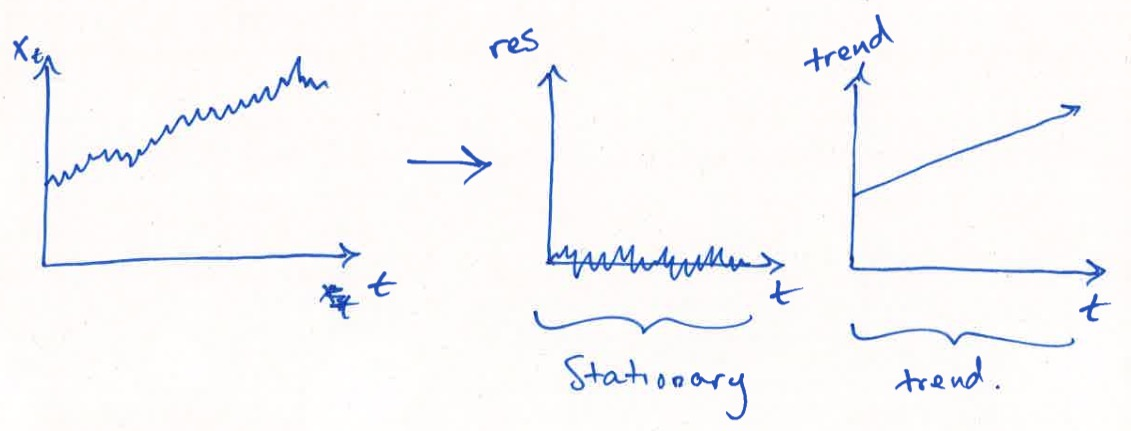
\includegraphics[scale=0.3]{images/Screenshot 2024-03-29 at 16.08.14.jpg}
\centering
\end{figure}

\subsubsection{Local Trend Extraction}

\textbf{\underline{Linear filtering}}: Transform $X_t$ into $Y_t$ according to \[Y_t = \sum_{r=-q}^S a_rX_{t+r}\] where $\{a_r\}$ is a set of weights. This operation is often called a moving average.\\

\textbf{Notation}: $Y_t=SM(X-t)$ \quad Sm="smoothed" \\

\textbf{Examples of Weight Schemes:}
\begin{itemize}
    \item Spencer's 15-point MA (moving average) with $q=7$:
    \[\{a_r\}=\frac{1}{320}(-3,-6,-5,3,27,46,67,74,67,...)\]
    \item Simple MA:
    \[a_r=\frac{1}{2q+1} \text{ for } r=-q,-q+1,...,q\]
\end{itemize}


\begin{figure}[H]
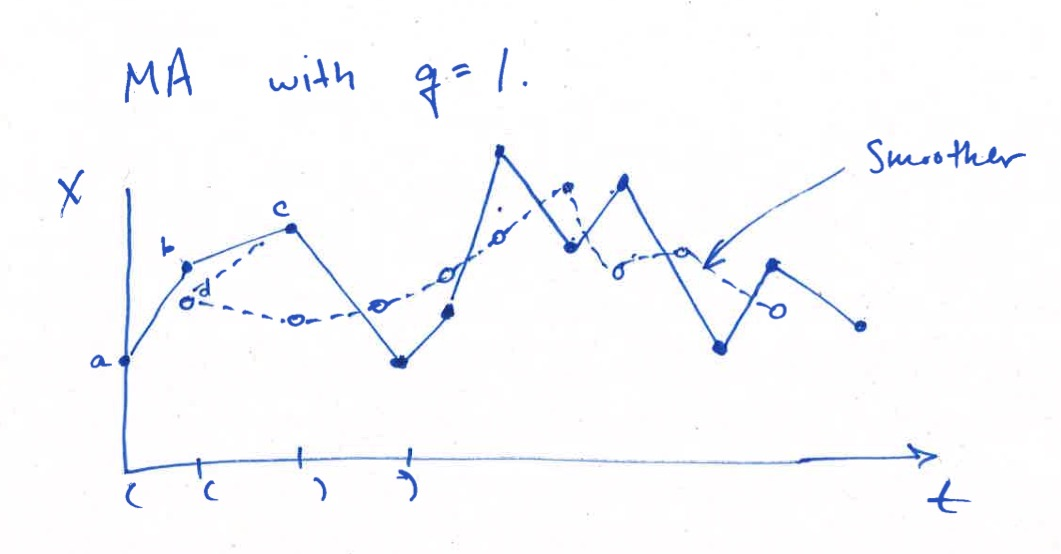
\includegraphics[scale=0.3]{images/Screenshot 2024-03-30 at 14.22.35.jpg}
\centering
\end{figure}


Again, like in Global trend extraction, for any linear filter, can calculate.
\[
\boxed{\text{res}(X_t)=X_t-\text{ Sm}(X_t)}
\]

\textbf{\underline{End effect problem}}: \\

If observed $ \{X_t\}_{t=1}^T $ cannot smooth forward at $X_T$. With simple MA with $q=1$, $Sm(X_t)=\frac{1}{3}(X_{t-1}+X_t+X_{t+1})$. Cannot calculate $Sm(X_T)$ as $X_{T+1}$ is unknown. \\

Can use asymmetric filters:
\[Sm(X_t)=\sum_{r=-q}^0 a_r X_t\]
$\Rightarrow X_{t+1}$ never affects $Sm(X_t)$
\begin{itemize}
    \item Exponential Smoothing $Sm(X_t)=\sum_{j=0}^\infty a(1-a)^j x_{t-j}$
    \item First Difference average $Sm(X_t)=\frac{1}{2}(X_t+X_{t-1})$
\end{itemize}


\textbf{\underline{Differencing}}:
\begin{itemize}
    \item \textbf{First Order Differencing}: $\nabla X_t = X_t - X_{t-1}$
    \item \textbf{Second Order Differencing}: $\nabla^2 X_t = \nabla \nabla X_t = \nabla (X_t- X_{t-1}) = \nabla X_t - \nabla X_{t-1} = X_t - 2X_{t-1} + X_{t-2}$
    \item \textbf{Seasonal Differencing}: $\nabla_2 = X_t - X_{t-2}$
    \item Seasonal + Second Order: $\nabla^2_2 X_t= \nabla_2 \nabla_2 X_t = \nabla_2 (X_t-X_{t-2}) = X_t - 2X_{t-2} + X_{t-4} $
\end{itemize}

\textbf{\underline{Kernel Smoothing}}\\

Any type of smoothing where weights are specified by a Kernel function. 
\[Sm(X_t)=\sum_{t'=1}^T w_t(t'), \quad w_t(t')= \frac{K\left(\frac{t-t'}{b} \right)}{\sum_{t''=1}^T K\left( \frac{t-t''}{b}\right)}\]

\begin{itemize}
    \item "Kernel function" $K$. \quad Example: $K(\cdot)=e^{\frac{-(\cdot)^2}{2}}$
    \item "Bandwidth $b$" number 
\end{itemize}

\textbf{\underline{Sequential filtering (Convolution)}}

\bigskip

\begin{itemize}
    \item First, filter $\{X_t\}$ with weights $\{a_r\}$ to obtain $\{y_t\}$
    \item Then, filter $\{y_t\}$ with weights $\{b_j\}$ to obtain $\{z_t\}$
    \item To get the 'combined' weights $\{c_k\}$:
        \[
        z_t=\sum_j b_j y_{t+j}=\sum_jb_j \sum_r a_r x_{t+j+r} = \sum_k c_k X_{t+k}, \quad \text{ where } c_k=\sum_r a_r b_{k-r}
        \]
\end{itemize}

\subsubsection{Detrending a Time Series}

\begin{figure}[H]
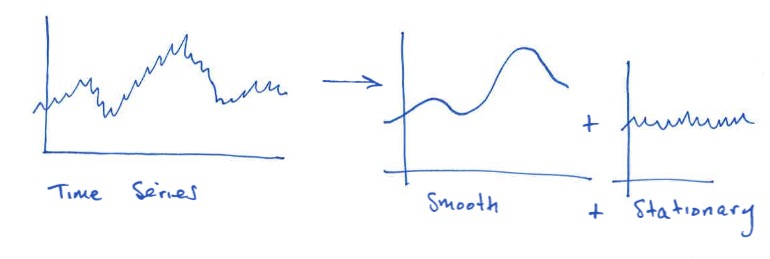
\includegraphics[scale=0.4]{images/Screenshot 2024-03-30 at 15.07.16.jpg}
\centering
\end{figure}

Global approach: Use a parametric functional form, e.g., $X_t=\beta t+\varepsilon_t$, $\beta$ estimated via least squares. \\

Local approach: Smoothing, $Y_t=Sm(X_t)=\sum_r a_r X_{t-r}$ \\

Detrending seasonality trends with local smoothing, e.g., the number of influenza cases recorded, is seasonal because there is a predictable peak in winter.\\

\textbf{Standard for Seasonality:}
\begin{align*}
    Y_t=Sm(X_t)&=\frac{0.5 X_{t-6} + X_{t-5}+...+X_{t+5} + 0.5 X_{t+6}}{12}\\
    Res(X_t)&=X_t-Sm(X_t) \quad \text{$\Rightarrow$ num. of surprise cases}
\end{align*}

Other procedures are available too, used by e.g., US Census Bureau:
\begin{itemize}
    \item X12 ARIMA
    \item SEATS-TRAMO
    \item X13 ARIMA-SEATS
\end{itemize}

\subsection{Autocorrelation and the Correlogram}

\textbf{Goal}: Come up with a method for measuring dependence between observations across time.\\

\subsubsection{Autocovariance Function}

The \textbf{autocovariance function (acv.f.)} measures the covariance between a time series and a lagged version of itself. For a time series $\{X_t\}$, the autocovariance function $\gamma(k)$ at lag $k$ is defined as:
\begin{align}
    \gamma(k)=Cov(X_t,X_{t+k})=\mathbb{E}\left[(X_t-\mu)(X_{t+k} -\mu) \right]
\end{align}
where $\mu$ is the mean of the time series.\\

Key properties of the acv.f. include:
\begin{itemize}
    \item $\gamma(0)$ is the variance of the time series
    \item $\gamma(k)=\gamma(-k)$ for all $k$ (i.e., the acv.f. is symmetric)
\end{itemize}

\subsubsection{Autocorrelation Function}

The \textbf{autocorrelation function (ac.f.)} measures the correlation between a time series and a lagged version of itself, normalizing the autocovariance function to ensure it lies between -1 and 1. The autocorrelation function $\rho(k)$ is defined as:
\begin{align}
    \rho(k)= \frac{\gamma(k)}{\gamma(0)}=\frac{\mathbb{E}[(X_t-\mu)(X_{t+k}-\mu)]}{\mathbb{E}[(X_t-\mu)^2]}
\end{align}

For a sample of size $T$, the sample autocorrelation function $r_k$ at lag $k$ is calculated as:

\begin{align}
    r_k=\frac{\sum_{t=1}^{T-k} (X_t-\bar{X})(X_{t+k}-\bar{X})}{\sum_{t=1}^{T} (X_t-\bar{X})^2}
\end{align}
where $\Bar{X}$ is the sample mean of the time series.


\textbf{Exc. 2.4 (Book)}: With a truly random process (under the assumption of a Gaussian white noise process) it is expected that the sample autocorrelation coefficient fall inside the C.I. that is given as: $\pm z\times \sqrt{\frac{1}{N}}$. (Note: in a random process it is normal to find some coefficient to fall just outside the C.I.)\\


\subsubsection{Correlogram}

A \textbf{correlogram} is a plot of the sample autocorrelation function values $r_k$ against the lag $k$. It is used to visualize the autocorrelation structure of a time series.

\begin{itemize}
    \item Choose a number $M<T$. E.g., if $T=200$, $M=30$ might be used
\end{itemize}

\begin{lstlisting}[language=R]
# In R (status package)
acf(x)        #(uses M=10*log_10(T))
                #(Horizontal bounds at +- 2/\sqrt(T) )
\end{lstlisting}

\textbf{Interpreting the Correlogram:}
\begin{itemize}
    \item If the series is white noise, the autocorrelation should be close to zero for all lags.
    \item Significant autocorrelation at non-zero lags indicate a possible underlying structure in the time series.
\end{itemize}

\textbf{Example:}

\begin{figure}[H]
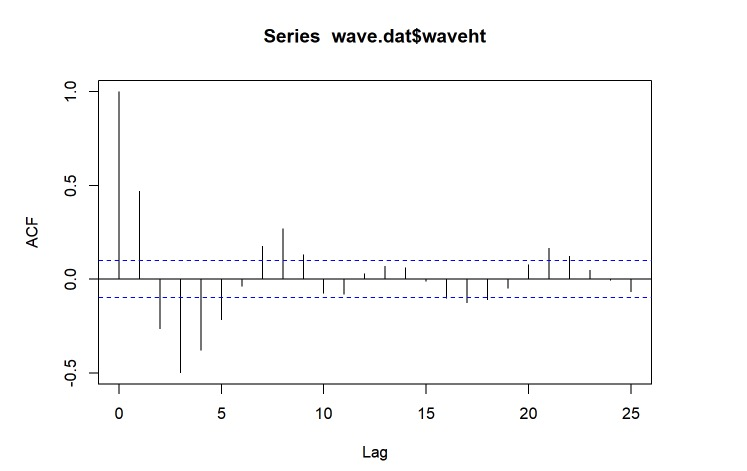
\includegraphics[scale=0.4]{images/Screenshot 2024-03-30 at 17.42.36.jpg}
\centering
\end{figure}


\subsection{Transformations}

In many cases, to reduce the unwanted effects of outliers, statistical routines can apply transformations to a time series.\\

Example:

\begin{figure}[H]
  \centering
  \begin{minipage}{0.49\textwidth}
    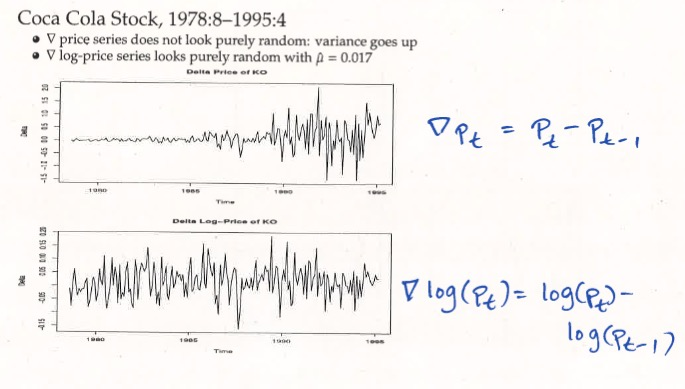
\includegraphics[height=5cm]{images/Screenshot 2024-03-30 at 17.45.04.jpg} % Left image
  \end{minipage}\hfill
  \begin{minipage}{0.49\textwidth}
    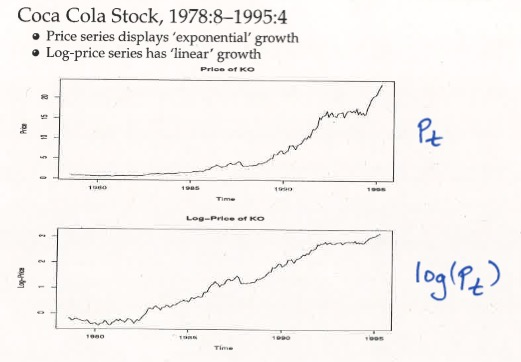
\includegraphics[height=5cm]{images/Screenshot 2024-03-30 at 17.46.58.jpg} % Right image
  \end{minipage}
\end{figure}

The three main reasons for making a transformation are:
\begin{enumerate}[label=(\roman*)]
    \item To stabilize the variance
    \item To make the seasonal effect additive
    \item To make the data normally distributed
\end{enumerate}

